\chapter{Mélange, oscillations, moments dipolaires électriques et opérateurs de champ}

Commençons par nous écarter un peu du sujet annoncé et poser une question sur les neutrinos. Des indices montrent que les neutrinos ont une masse et que leurs types se mélangent. Si leurs masses ne sont pas toutes identiques, comment un type peut-il se transformer en un autre sans violer la conservation de l’énergie ?

Cette question nous mène à un phénomène récurrent en mécanique quantique : les états dans lesquels un système est préparé ou détecté ne sont pas nécessairement ceux qui diagonalisent son hamiltonien. Un état d’énergie définie ne fait qu’acquérir une phase. En revanche, un état préparé comme superposition de plusieurs énergies évolue parce que ses composantes acquièrent des phases différentes. Cette distinction nous conduira du double puits aux oscillations des neutrinos et à la précession du spin. Après une parenthèse consacrée au moment dipolaire électrique de l’électron, nous reviendrons à la seconde quantification et retrouverons la même structure de Fourier position--impulsion au niveau des opérateurs.

\section{Le véritable enjeu : le mélange}

Les neutrinos n’ont pas nécessairement tous la même masse. Les états propres d’énergie ne se mélangent pas entre eux : chacun évolue indépendamment. Ce que nous appelons le \emph{type} ou la saveur d’un neutrino est lié à la façon dont il est produit et détecté ; un état de saveur peut être une combinaison linéaire d’états propres de masse et d’énergie. Schématiquement, \begin{equation}
|\text{type}\rangle = \sum_n c_n |E_n\rangle .
\end{equation}La bonne formulation n’est donc pas que les états propres d’énergie se transforment les uns en les autres, mais que les états appelés ``neutrino électronique'' ou ``neutrino muonique'' ne sont pas nécessairement eux-mêmes des états propres d’énergie.

\begin{classroomqa}\lecturetimestamp{00:00:09}\audiencequestion{Si les neutrinos ont des masses différentes, comment peuvent-ils se mélanger alors que l’énergie se conserve ?}\lecturerresponse{Les états propres de masse et d’énergie ne se transforment pas les uns en les autres. Les états de saveur électronique, muonique et tauique sont différentes combinaisons linéaires de ces états propres. Chaque composante de masse évolue avec sa propre phase, et l’interférence modifie les probabilités de saveur sans violer la conservation de l’énergie.}\end{classroomqa}

Cette structure se retrouve dans de nombreux exemples. Le plus parlant commence par une particule dans un double puits symétrique.

\section{Puits double symétrique et états approximativement localisés}

Considérons une particule dans un potentiel symétrique à double puits, avec une barrière élevée entre les deux minima. Si la hauteur de la barrière était infinie, les puits gauche et droit seraient complètement découplés. On pourrait résoudre le problème dans le puits de gauche comme si celui de droite n’existait pas, et réciproquement. Les fonctions d’onde approchées de l’état fondamental seraient alors un état localisé à gauche \(\psi_L\) et un état localisé à droite \(\psi_R\), tous deux d’énergie \(E\).

Dans chaque puits isolé, l’état fondamental possède les propriétés qualitatives habituelles : il est lisse, sans nœud, et se situe à l’énergie la plus basse compatible avec le confinement. Imaginons que la haute barrière centrale soit un mur de briques. La traiter comme infinie n’est qu’une approximation, mais elle nous fournit une paire utile d’états localisés pour commencer.

\begin{figure}\centering
\begin{adjustbox}{max width=\linewidth}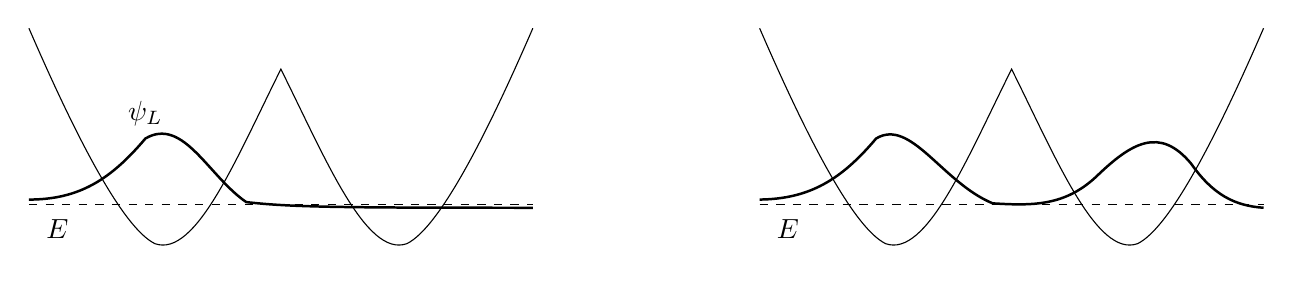
\begin{tikzpicture}[x=0.8cm,y=0.8cm]
\begin{scope}[shift={(-5.8,0)}]
\draw (-4,2.7) .. controls (-3.35,1.2) and (-2.55,-0.45) .. (-2.0,-0.72)
      .. controls (-1.35,-0.95) and (-0.7,0.65) .. (0,2.05)
      .. controls (0.7,0.65) and (1.35,-0.95) .. (2.0,-0.72)
      .. controls (2.55,-0.45) and (3.35,1.2) .. (4,2.7);
\draw[dashed] (-4,-0.10) -- (4,-0.10);
\node at (-3.55,-0.48) {$E$};
\draw[line width=0.9pt] (-4,-0.02) .. controls (-3.2,-0.02) and (-2.7,0.30) .. (-2.15,0.95)
      .. controls (-1.55,1.30) and (-1.15,0.35) .. (-0.55,-0.06)
      .. controls (0.15,-0.14) and (0.9,-0.15) .. (4,-0.15);
\node at (-2.15,1.35) {$\psi_L$};
\end{scope}
\begin{scope}[shift={(5.8,0)}]
\draw (-4,2.7) .. controls (-3.35,1.2) and (-2.55,-0.45) .. (-2.0,-0.72)
      .. controls (-1.35,-0.95) and (-0.7,0.65) .. (0,2.05)
      .. controls (0.7,0.65) and (1.35,-0.95) .. (2.0,-0.72)
      .. controls (2.55,-0.45) and (3.35,1.2) .. (4,2.7);
\draw[dashed] (-4,-0.10) -- (4,-0.10);
\node at (-3.55,-0.48) {$E$};
\draw[line width=0.9pt] (-4,-0.02) .. controls (-3.2,-0.01) and (-2.7,0.30) .. (-2.15,0.95)
      .. controls (-1.6,1.28) and (-1.1,0.25) .. (-0.30,-0.08)
      .. controls (0.35,-0.12) and (0.85,-0.12) .. (1.35,0.35)
      .. controls (1.9,0.88) and (2.35,1.15) .. (2.85,0.55)
      .. controls (3.2,0.05) and (3.55,-0.12) .. (4,-0.15);
\end{scope}
\end{tikzpicture}\end{adjustbox}\caption{Redessin soigné des schémas d’ouverture au tableau. À gauche figure l’état d’essai unilatéral \(\psi_L\), obtenu en faisant comme si la barrière était effectivement infinie. À droite, la même fonction d’onde est prolongée symétriquement à travers la barrière, illustrant la faible fuite, non nulle, qui donnera finalement le véritable état fondamental pair.}\end{figure}

En mécanique quantique, toutefois, la barrière n’est pas réellement infinie. La fonction d’onde dans la région de la barrière n’est pas exactement nulle ; elle est seulement très petite. Toute l’histoire tient à cette infime fuite. C’est elle qui transforme l’approximation gauche-droite en un véritable problème de mélange.

\section{États propres de parité et dédoublement exponentiellement faible des niveaux}

Le tableau des états localisés est maintenant interrompu par un théorème : si le potentiel est symétrique, on peut choisir les fonctions propres exactes de l’énergie de sorte qu’elles soient soit symétriques, soit antisymétriques par réflexion.

\begin{theorem}Si \(V(x)=V(-x)\) en une dimension, les fonctions propres de l’hamiltonien peuvent être choisies de sorte à satisfaire l’une ou l’autre des relations suivantes : \[
\psi(x)=\psi(-x)
\qquad \text{or} \qquad
\psi(x)=-\psi(-x).
\]\end{theorem}

Voici maintenant la correction. Les états unilatéraux \(\psi_L\) et \(\psi_R\) ne sont ni symétriques ni antisymétriques ; ils ne peuvent donc pas être des états propres exacts de l’hamiltonien complet. Ce ne sont que de bons états approchés lorsque la barrière est élevée. Les véritables états propres sont les combinaisons symétrique et antisymétrique, \begin{align}
\psi_+ &= \frac{\psi_L+\psi_R}{\sqrt{2}},\\
\psi_- &= \frac{\psi_L-\psi_R}{\sqrt{2}}.
\end{align}En notant leurs énergies comme elles le seront au tableau, on a \begin{align}
H\psi_+ &= (E_1-\epsilon)\psi_+,\\
H\psi_- &= (E_1+\epsilon)\psi_-.
\end{align}L’écart total vaut donc \begin{equation}
\Delta E = (E_1+\epsilon)-(E_1-\epsilon)=2\epsilon .
\end{equation}

\begin{figure}[htbp]\centering
\includegraphics[width=0.92\linewidth]{lecture_08_frame_02.png}\caption{La fonction d’onde prolongée symétriquement dans le potentiel à double puits. Son amplitude sous la barrière est faible mais non nulle, ce qui est à l’origine de la séparation des niveaux.}\lectureframe{00:06:19}\end{figure}

\begin{figure}\centering
\begin{tikzpicture}[x=1cm,y=1cm]
\draw[->] (0,0) -- (0,3);
\node[left] at (0,2.8) {energy};
\draw (-0.35,1.60) -- (0.35,1.60);
\node[left] at (-0.45,1.60) {$\psi_L,\psi_R$};
\node at (1.7,1.60) {$\Longrightarrow$};
\draw (3.0,1.32) -- (3.75,1.32);
\draw (3.0,1.88) -- (3.75,1.88);
\draw[dashed] (2.8,1.60) -- (3.95,1.60);
\node[right] at (3.9,1.32) {$\psi_+,\ E_1-\epsilon$};
\node[right] at (3.9,1.88) {$\psi_-,\ E_1+\epsilon$};
\node[below] at (3.37,1.60) {$E_1$};
\end{tikzpicture}\caption{Schéma au tableau de la séparation par effet tunnel. Les états approchés gauche et droit sont presque dégénérés, mais les états propres exacts symétrique et antisymétrique sont séparés par une petite quantité \(2\epsilon\).}\end{figure}

L’ordre des niveaux porte en lui le point physique. L’état symétrique est légèrement plus bas en énergie, car il est plus lisse dans la région de la barrière ; le fait que la fonction d’onde puisse fuir et se prolonger symétriquement abaisse l’énergie d’une petite quantité. L’état antisymétrique est légèrement plus haut : en une dimension, le premier état excité possède un nœud, qui, dans ce problème symétrique, se trouve au milieu. Une courbure supplémentaire coûte de l’énergie cinétique.

L’effet est très faible, exponentiellement faible en fonction de la largeur et de la hauteur de la barrière. Il n’est pas nécessaire d’écrire ici une formule WKB explicite ; l’essentiel est que la séparation existe, mais qu’elle est minuscule. Rappelons aussi que le signe global d’une fonction d’onde n’a pas de signification physique. Remplacer \(\psi_-\) par \(-\psi_-\) ne change pas l’état.

\section{Évolution temporelle et oscillation gauche-droite}

Posons maintenant la question dynamique : que se passe-t-il si l’on place une particule dans le puits de gauche ? C’est l’étape décisive, car l’oscillation est la manifestation temporelle du même phénomène de mélange.

Les relations inverses sont \begin{align}
\psi_L &= \frac{\psi_+ + \psi_-}{\sqrt{2}},\\
\psi_R &= \frac{\psi_+ - \psi_-}{\sqrt{2}}.
\end{align}Un état initialement localisé à gauche s’écrit donc \begin{equation}
\psi(0)=\psi_L=\frac{\psi_+ + \psi_-}{\sqrt{2}}.
\end{equation}Ce n’est pas un état propre d’énergie ; il doit donc évoluer de façon non triviale.

Nous adoptons la convention standard de Schr\"odinger\(e^{-iEt}\). Une phase commune n’a aucun effet observable ; seule la phase relative entre les deux composantes d’énergie peut transférer la probabilité d’un puits à l’autre.

Avec cette convention, \begin{equation}
\psi(t)=\frac{1}{\sqrt{2}}\left(e^{-i(E_1-\epsilon)t}\psi_+ + e^{-i(E_1+\epsilon)t}\psi_-\right).
\end{equation}Voici la formule du tableau mise au propre. Factorisons maintenant la phase commune : \begin{equation}
\psi(t)=\frac{e^{-iE_1 t}}{\sqrt{2}}\left(e^{i\epsilon t}\psi_+ + e^{-i\epsilon t}\psi_-\right).
\end{equation}Une phase évolue dans un sens autour du cercle unité, tandis que l’autre évolue en sens inverse. L’état ne change que parce que ces deux phases se décalent l’une par rapport à l’autre.

Pour faire apparaître explicitement l’oscillation gauche-droite, substituons les définitions de \(\psi_\pm\) : \begin{align}
\psi(t)
&= \frac{e^{-iE_1 t}}{2}
\left[e^{i\epsilon t}(\psi_L+\psi_R)+e^{-i\epsilon t}(\psi_L-\psi_R)\right] \\
&= \frac{e^{-iE_1 t}}{2}
\left[(e^{i\epsilon t}+e^{-i\epsilon t})\psi_L+(e^{i\epsilon t}-e^{-i\epsilon t})\psi_R\right] \\
&= e^{-iE_1 t}\left[\psi_L\cos(\epsilon t)+i\,\psi_R\sin(\epsilon t)\right].
\end{align}Voici la dérivation centrale de ce chapitre. Dans l’approximation à deux états, avec \(\psi_L\) et \(\psi_R\) orthonormés, les probabilités sont \begin{equation}
P_L(t)=\cos^2(\epsilon t),
\qquad
P_R(t)=\sin^2(\epsilon t).
\end{equation}Le système oscille donc. Aux temps intermédiaires, il se trouve véritablement dans une superposition ; par exemple, lorsque \(\epsilon t=\pi/4\), les probabilités de présence dans les deux puits sont égales. Les phases évoluent continûment, et la localisation change continûment avec elles.

La dérivation au tableau isole le premier instant où le signe relatif s’inverse. On cherche quand \begin{equation}
e^{-i\epsilon t}=-\,e^{i\epsilon t},
\end{equation}ce qui constitue le repère visible au tableau. En multipliant les deux membres, on obtient \begin{equation}
e^{2i\epsilon t}=-1.
\end{equation}Pour la première occurrence, \begin{equation}
2\epsilon t=\pi,
\qquad\text{so}\qquad
t_{L\to R}=\frac{\pi}{2\epsilon}.
\end{equation}

\begin{figure}[htbp]\centering
\includegraphics[width=0.94\linewidth]{lecture_08_frame_05.png}\caption{Calcul de la phase relative au tableau. Les deux composantes d’énergie deviennent opposées lorsque \(e^{2i\epsilon t}=-1\), ce qui donne le premier temps de transfert \(2\epsilon t=\pi\). La dérivation mise en forme adopte une convention de phase de Schr\"odinger cohérente.}\lectureframe{00:17:52}\end{figure}À cet instant, \begin{equation}
\psi(t_{L\to R}) \propto \frac{\psi_+-\psi_-}{\sqrt{2}}=\psi_R.
\end{equation}La phase globale est sans importance. Ce qui compte, c’est que la particule placée initialement à gauche a évolué vers l’état localisé à droite. Après le même intervalle de temps, elle revient en sens inverse. Mélange et oscillation vont de pair.

L’équation ne laisse aucun doute : une petite valeur de \(\epsilon\) implique une oscillation lente et un temps de transfert long. Aucun des deux états localisés n’a une énergie définie, mais les deux composantes d’énergie exactes conservent l’énergie et évoluent exactement comme elles le doivent.

\section{Analogies avec les neutrinos, l’ammoniac et le spin}

Le double puits nous donne un modèle pour aborder la question initiale sur les neutrinos. Un neutrino créé en même temps qu’un électron est appelé neutrino électronique ; s’il est créé en même temps qu’un muon, on parle de neutrino muonique. Ces étiquettes de saveur décrivent les canaux de production et de détection. Les états de masse définie, et donc d’énergie définie à impulsion fixée pour une particule libre, forment une autre base.

Dans une caricature simple à deux états avec mélange maximal, \begin{equation}
|\nu_e\rangle \sim \frac{|m_1\rangle+|m_2\rangle}{\sqrt{2}},
\qquad
|\nu_\mu\rangle \sim \frac{|m_1\rangle-|m_2\rangle}{\sqrt{2}},
\end{equation}les états propres de masse jouent le rôle de \(\psi_+\) et \(\psi_-\), tandis que les états de saveur jouent celui de \(\psi_L\) et \(\psi_R\). Le mélange réel des neutrinos fait intervenir une matrice de mélange aux coefficients différents, mais le mécanisme apparaît déjà ici.

Un neutrino électronique est produit dans un processus faisant intervenir un électron, tout comme une particule peut être déposée dans le puits de gauche. Sur un trajet court, ses deux composantes de masse ont accumulé presque la même phase ; une interaction l’identifie donc toujours comme étant de saveur électronique. Sur une longue distance, leurs phases se séparent. Une interaction à courant chargé ultérieure peut alors produire un muon plutôt qu’un électron : l’état a acquis une composante de saveur muonique. La répétition de l’expérience à différentes distances ou énergies met en évidence l’oscillation.

Il n’y a aucune contradiction avec la conservation de l’énergie. Les états propres de masse et d’énergie se comportent bien comme des états propres. C’est la superposition de saveurs qui évolue. À la limite relativiste, la phase relative observable est gouvernée par les différences des carrés des masses ; schématiquement, \begin{equation}
\Delta\phi_{ij}\simeq \frac{\Delta m_{ij}^{,2}L}{2E}.
\end{equation}Les oscillations montrent donc que les masses des neutrinos ne sont pas toutes identiques : au moins deux états propres de masse ont des masses différentes.

\begin{classroomqa}\lecturetimestamp{00:24:06}\audiencequestion{De quoi dépend la faible séparation \(\epsilon\) dans l’exemple du double puits ?}\lecturerresponse{Elle dépend de la masse de la particule ainsi que de la hauteur et de la largeur de la barrière. L’effet tunnel est exponentiellement sensible à ces paramètres ; une variation modérée de la barrière peut donc entraîner une forte variation relative de \(\epsilon\).}\end{classroomqa}

\begin{classroomqa}\lecturetimestamp{00:24:26}\audiencequestion{Ce phénomène d’oscillation a-t-il réellement été observé ?}\lecturerresponse{Oui. Les séparations par effet tunnel sont observées dans des systèmes quantiques ordinaires, et les oscillations de saveur sont observées pour les neutrinos. Les mécanismes diffèrent à l’échelle microscopique, mais les deux réalisent la même évolution de phase à deux états.}\end{classroomqa}

\begin{classroomqa}\lecturetimestamp{00:24:34}\audiencequestion{Quel est le lien entre les oscillations des neutrinos et leur masse ?}\lecturerresponse{Les états propres qui se propagent ont des masses différentes et accumulent donc des phases différentes. Leur interférence modifie la composition en saveur. Dans un traitement relativiste réaliste, ce sont les différences des carrés des masses, et non une masse de la particule qui varierait littéralement dans le temps, qui déterminent l’oscillation.}\end{classroomqa}

\begin{classroomqa}\lecturetimestamp{00:25:02}\audiencequestion{La masse des neutrinos est-elle simplement une théorie dominante ou un fait expérimental ?}\lecturerresponse{Les oscillations sont un fait expérimental et exigent des différences de masse non nulles. L’échelle absolue des masses est une mesure distincte et plus difficile, mais les expériences excluent le modèle minimal où tous les neutrinos seraient sans masse.}\end{classroomqa}

\subsection{Inversion de l’ammoniac : une barrière bien réelle}

Une molécule d’ammoniac, \(\mathrm{NH}_3\), a une géométrie pyramidale trigonale : les trois atomes d’hydrogène forment un plan et l’atome d’azote se trouve d’un côté de celui-ci. Il existe une configuration équivalente où l’azote se trouve de l’autre côté. Ces deux configurations localisées ne sont pas des états stationnaires exacts. L’azote peut traverser par effet tunnel le plan des atomes d’hydrogène, ce qui produit des états propres d’énergie symétrique et antisymétrique, ainsi qu’une faible séparation d’inversion. C’est l’origine physique de ces mêmes mathématiques dans le maser à ammoniac.

\begin{classroomqa}\lecturetimestamp{00:25:11}\audiencequestion{Dans l’ammoniac, la barrière correspond-elle à la configuration où l’azote traverse le plan des atomes d’hydrogène ?}\lecturerresponse{Oui. L’énergie moléculaire est minimale dans chacune des deux configurations pyramidales, tandis que la configuration plane est plus élevée en énergie. Le passage par effet tunnel à travers cette configuration couple les deux côtés.}\end{classroomqa}

\begin{classroomqa}\lecturetimestamp{00:27:10}\audiencequestion{Quelle est la barrière physique correspondante entre les neutrinos électroniques et muoniques ?}\lecturerresponse{Il n’existe pas de barrière spatiale au sens littéral. L’analogie est algébrique : un couplage hors diagonale dans l’hamiltonien des neutrinos mélange la base de saveur. Dans l’ammoniac, ce couplage provient de l’effet tunnel ; pour les neutrinos, il fait partie de la structure de masse et de mélange.}\end{classroomqa}

\subsection{Précession du spin : mélange sans effet tunnel}

Nous avons déjà rencontré la même algèbre avec le spin. Considérons les deux états \(|\uparrow_z\rangle\) et \(|\downarrow_z\rangle\). En l’absence de champ magnétique, ils sont dégénérés. Appliquons maintenant un champ magnétique dirigé selon \(x\). Les états propres d’énergie ne sont plus les états propres de \(z\), mais les états polarisés selon \(x\). En utilisant provisoirement les appellations gauche--droite du tableau, \begin{align}
|L_x\rangle &= \frac{|\uparrow_z\rangle+|\downarrow_z\rangle}{\sqrt{2}},\\
|R_x\rangle &= \frac{|\uparrow_z\rangle-|\downarrow_z\rangle}{\sqrt{2}}.
\end{align}Ce sont les analogues directs de \(\psi_+\) et \(\psi_-\). Les moments magnétiques aligné et antialigné sur le champ ont des énergies légèrement différentes. Si ces énergies sont \(E\mp\epsilon\), un spin initialement orienté vers le haut évolue comme suit : \begin{equation}
|\uparrow_z,t\rangle
= e^{-iEt}\left[\cos(\epsilon t)\,|\uparrow_z\rangle
+ i\sin(\epsilon t)\,|\downarrow_z\rangle\right].
\end{equation}C’est la même formule que pour le double puits ; cette fois, l’évolution continue est une précession du spin autour de l’axe \(x\). Partant de \(+z\), le spin passe par des directions transversales, atteint \(-z\) au bout d’une demi-période de précession, puis revient après une autre demi-période. Une mesure de \(S_z\) ne donne toujours que « vers le haut » ou « vers le bas » ; c’est l’évolution continue de l’état de spin qui détermine les probabilités. Ce mécanisme ne nécessite pas d’effet tunnel. Il suffit que l’hamiltonien soit diagonal dans une base différente de celle de préparation.

\begin{classroomqa}\lecturetimestamp{00:32:25}\audiencequestion{Dans cette représentation, qu’advient-il du neutrino tauique ?}\lecturerresponse{Il se mélange lui aussi. Le problème réel comporte trois états de saveur et trois états de masse ; une matrice de mélange trois par trois remplace donc la rotation à deux états. Le principe d’interférence des phases reste inchangé.}\end{classroomqa}

\begin{classroomqa}\lecturetimestamp{00:32:57}\audiencequestion{Juste après l’application du champ transverse, le spin est-il encore orienté vers le haut, et peut-il pointer vers nous ou dans la direction opposée ?}\lecturerresponse{Au bout d’un temps très court, il est encore presque certainement orienté vers le haut, avec une faible probabilité de le trouver vers le bas. L’état précesse continûment autour de l’axe du champ et passe par les directions transversales \(\pm y\), tout en restant perpendiculaire au champ dirigé selon \(x\) s’il était initialement perpendiculaire. Une mesure le long d’un axe choisi donne toujours l’une des valeurs propres discrètes associées à cet axe.}\end{classroomqa}

\begin{classroomqa}\lecturetimestamp{00:34:30}\audiencequestion{Le champ est-il choisi faible pour que le spin ne pointe jamais dans sa direction ?}\lecturerresponse{Non. La géométrie résulte de la précession autour de l’axe du champ, et non de la faiblesse de celui-ci. Un champ faible réduit simplement la séparation des énergies et la fréquence de précession, produisant une oscillation lente analogue à l’exemple des neutrinos.}\end{classroomqa}

L’origine profonde de l’intensité du mélange des neutrinos et de leurs faibles masses n’est pas expliquée par le modèle standard minimal tel qu’il a été formulé à l’origine. La masse des neutrinos indique donc que ce modèle minimal est incomplet, même si l’échelle observée est très faible et peut refléter une physique à une échelle d’énergie très éloignée.

\begin{classroomqa}\lecturetimestamp{00:36:27}\audiencequestion{Est-ce grâce aux oscillations que nous savons que les neutrinos ont une masse ?}\lecturerresponse{C’est l’indice direct décisif que les composantes qui se propagent ont des masses différentes. Si toutes les composantes pertinentes étaient exactement sans masse et dégénérées, elles n’accumuleraient aucune phase relative dépendant de la masse et il n’y aurait pas d’oscillation de saveur dans le vide de ce type.}\end{classroomqa}

\begin{classroomqa}\lecturetimestamp{00:37:57}\audiencequestion{À la moitié d’une période, un neutrino devrait-il se comporter à moitié comme un neutrino électronique et à moitié comme un neutrino muonique ?}\lecturerresponse{Dans le modèle idéal symétrique à deux états, les probabilités sont égales au quart de la période complète des probabilités, tandis que la conversion totale se produit au premier maximum. Les oscillations réelles à trois saveurs comportent des angles de mélange inégaux, plusieurs fréquences, des contraintes liées au spin et à l’hélicité, ainsi que des effets de matière ; une conversion symétrique complète n’est donc pas générique.}\end{classroomqa}

\begin{classroomqa}\lecturetimestamp{00:38:36}\audiencequestion{Si les composantes de masse diffèrent, la vitesse d’un neutrino solaire doit-elle changer pour que l’impulsion se conserve ?}\lecturerresponse{Un état de saveur est une superposition cohérente de composantes de masses fixes ; sa masse n’est pas une grandeur classique qui oscille dans le temps. Dans la description courante à impulsion égale, les composantes ont des énergies et des vitesses de groupe légèrement différentes ; dans une description à énergie égale, elles ont des impulsions légèrement différentes. Les deux conventions donnent la même phase d’oscillation observable si elles sont appliquées de façon cohérente.}\end{classroomqa}

Cette évolution de phase a résolu l’ancienne énigme du déficit de neutrinos solaires. Les premiers détecteurs étaient principalement sensibles aux neutrinos électroniques ; des neutrinos ayant quitté le Soleil avec une saveur électronique pouvaient donc arriver en partie avec une saveur muonique ou tauique et échapper à ce canal de détection. Le calcul détaillé du Soleil inclut le mélange à trois saveurs et les effets de matière, mais la leçon conceptuelle est déjà présente dans le double puits : la préparation et la propagation font appel à des bases différentes.

\section{Interlude : moment dipolaire électrique, symétrie et affirmation de la ``sphère de l’électron''}

Puisque nous parlons déjà de phénoménologie des particules, faisons une pause dans les développements mathématiques. Un article populaire a présenté une nouvelle limite sur le moment dipolaire électrique de l’électron en affirmant qu’on avait montré que l’électron était une sphère. Ce slogan confond trois questions distinctes : ce que mesure un moment dipolaire électrique, ce que signifie la symétrie de rotation pour un état quantique et ce que l’expérience a effectivement contraint.

\subsection{Qu’a-t-on mesuré ?}

Ce qui a été mesuré, ou plutôt ce dont on a établi une borne, c’est le moment dipolaire électrique de l’électron. Pour des charges séparées \(\pm q\), le moment dipolaire est \begin{equation}
\mathbf d = q\,\boldsymbol{\ell},
\end{equation}où \(\boldsymbol{\ell}\) est le vecteur séparation. Un moment dipolaire non nul signifie que la distribution de charge est décalée par rapport à un certain centre.

Pour l’électron, toutefois, la question pertinente n’est pas simplement de savoir si la charge est décentrée dans une direction arbitraire. L’électron possède un spin, donc un axe. Il possède aussi un moment magnétique. La question physiquement pertinente est de savoir s’il existe une corrélation entre le déplacement de la charge et cet axe : \begin{equation}
\mathbf d_e \parallel \boldsymbol{\mu}_e
\qquad \text{or equivalently} \qquad
\mathbf d_e \parallel \mathbf S .
\end{equation}C’est ce que l’on entend par moment dipolaire électrique de l’électron. Conceptuellement, on cherche à savoir si placer un électron polarisé en spin dans un champ électrique sépare les deux orientations du spin : \begin{equation}
H_{\mathrm{EDM}}=-\mathbf d_e\cdot \mathbf E,
\qquad
\mathbf d_e=d_e\frac{\mathbf S}{|\mathbf S|}.
\end{equation}L’expérience de table réelle est bien plus subtile qu’un électron nu placé entre les plaques d’un condensateur, mais elle exploite cette idée de symétrie et de décalage d’énergie.

\subsection{Pourquoi l’absence de moment dipolaire électrique ne signifie pas que l’électron est sphérique}

La première correction est élémentaire. Un corps peut avoir un moment dipolaire nul sans être sphérique. Un ellipsoïde centré possède autant de charge d’un côté que de l’autre et n’a donc pas de dipôle, mais il peut avoir un moment quadrupolaire. Une distribution plus complexe peut n’avoir ni dipôle ni quadrupôle tout en présentant des multipôles d’ordre supérieur. Mesurer un coefficient multipolaire ne détermine pas une forme entière.

La mécanique quantique rend le mot ``forme'' plus délicat. Imaginons une molécule en forme d’haltère composée de deux atomes, dont la longueur de liaison est approximativement fixe. Négligeons les vibrations radiales et ne considérons que les rotations. Ses états de rotation sont caractérisés par le moment cinétique. Si la molécule est bosonique, l’état de rotation le plus bas a \(J=0\). Comme le moment cinétique engendre les rotations, \begin{equation}
\begin{gathered}
J=0 \quad\Longrightarrow\\
\text{rotationally invariant ground state.}
\end{gathered}
\end{equation}L’état quantique est invariant par rotation, même si toute représentation à orientation définie ressemble à un haltère. On peut le décrire comme une superposition cohérente de toutes les orientations. Qualifier l’état de ``sphérique'' est utile pour certaines mesures et trompeur pour d’autres.

Prenons un instantané. Un instantané est une mesure de l’orientation et une mesure de l’orientation suffisamment précise laisse le système dans un état localisé angulairement. Un tel état ne peut pas avoir en même temps un moment cinétique défini. C’est la version rotationnelle du principe d’incertitude position--impulsion : localiser l’angle implique nécessairement une dispersion des moments cinétiques et donc une excitation rotationnelle.

Pour un rotor rigide, \begin{equation}
E_J=\frac{J(J+1)}{2I},
\end{equation}l’énergie nécessaire à la résolution est donc déterminée par le moment d’inertie \(I\). Un haltère de gymnastique a un \(I\) énorme et des niveaux de rotation incroyablement rapprochés ; la lumière ordinaire peut facilement le perturber assez pour révéler une orientation. Les niveaux d’une molécule sont plus espacés. Ceux d’un hadron compact le sont davantage encore. Si la sonde n’a pas assez d’énergie pour exciter la première structure rotationnelle résoluble, des mesures répétées ne voient que l’état fondamental moyenné sur les rotations.

On peut se représenter grossièrement un méson comme un système à deux corps quark--antiquark. Ses premières excitations orbitales coûtent des centaines de millions d’électronvolts, voire davantage, bien plus qu’un photon optique. Une sonde de faible énergie ne peut donc pas prendre un instantané de l’orientation sous-jacente. ``La question de savoir s’il est sphérique'' dépend en partie de l’état préparé et en partie de la résolution de l’appareil.

Le cas de l’électron rend la question plus précise. C’est une particule de spin \(\tfrac12\), et non un scalaire de rotation. Un état polarisé en spin porte un axe et un moment magnétique. L’image familière d’une charge circulant autour de cet axe n’est qu’une heuristique---une particule de Dirac ponctuelle n’est pas littéralement une minuscule boule en rotation---mais elle nous rappelle à juste titre que le moment magnétique s’inverse lorsque le spin s’inverse. La question du moment dipolaire électrique est de savoir si le déplacement de la charge électrique est corrélé à ce même axe. Une réponse nulle ne transforme pas l’électron en sphère classique.

\begin{classroomqa}\lecturetimestamp{00:57:30}\audiencequestion{Déplacer une partie de la charge de l’électron violerait-il la quantification de la charge ?}\lecturerresponse{Non. La quantification de la charge fixe la charge totale. Un moment dipolaire concerne le premier moment spatial de cette distribution de charge, ou, de manière équivalente, un couplage ponctuel permis au champ électrique ; il n’implique pas de fractionner la charge totale.}\end{classroomqa}

\begin{classroomqa}\lecturetimestamp{00:58:00}\audiencequestion{Les moments dipolaires électriques sont-ils interdits par la théorie quantique des champs ?}\lecturerresponse{La théorie quantique des champs ne les interdit pas en elle-même. Ils sont interdits lorsque certaines symétries discrètes sont exactes. Dès lors que ces symétries sont violées, un opérateur de moment dipolaire électrique est permis, même si son coefficient peut être extrêmement faible.}\end{classroomqa}

\subsection{Parité et renversement du temps}

Le véritable enjeu de la discussion sur le moment dipolaire électrique est la symétrie. Sous l’action de la parité, un moment dipolaire électrique se transforme comme un vecteur polaire ordinaire, tandis qu’un moment magnétique se transforme comme un vecteur axial : \begin{align}
P:\qquad &\mathbf d_e \to -\mathbf d_e,
&\boldsymbol{\mu}_e \to \boldsymbol{\mu}_e .
\end{align}Sous l’action du renversement du temps, le courant circulant qui définit le moment magnétique s’inverse, contrairement à un déplacement électrostatique : \begin{align}
T:\qquad &\mathbf d_e \to \mathbf d_e,
&\boldsymbol{\mu}_e \to -\boldsymbol{\mu}_e .
\end{align}Par conséquent, un moment dipolaire électrique non nul aligné sur l’axe du spin de l’électron est interdit si la symétrie de parité est exacte, et également si la symétrie de renversement du temps est exacte : \begin{equation}
(P\ \text{exact}) \Rightarrow \mathbf d_e=0,
\qquad
(T\ \text{exact}) \Rightarrow \mathbf d_e=0.
\end{equation}

Il vaut la peine de préciser la géométrie. Un moment magnétique est produit par un courant circulant dans une boucle. La réflexion par parité inverse les vecteurs polaires ordinaires, mais laisse inchangé le vecteur axial normal à cette boucle. Un déplacement de charge le long de l’axe, lui, est inversé. Ainsi, un électron dont \(\mathbf d_e\) est parallèle à \(\boldsymbol\mu_e\) serait transformé par la parité en un électron ayant la même orientation magnétique, mais une relation opposée entre ses moments électrique et magnétique. Si la parité était une symétrie exacte et qu’il n’existait qu’une seule espèce d’électron, ces deux descriptions devraient représenter la même particule ; seule la condition \(d_e=0\) est compatible avec cela.

L’inversion du temps conduit à la même conclusion d’une autre manière. Passer le film à l’envers inverse le courant et donc \(\boldsymbol\mu_e\), mais ne déplace pas un déplacement de charge statique. Un état où les moments sont parallèles devient un état où ils sont antiparallèles. Une symétrie exacte par renversement du temps exigerait donc, là encore, que \(d_e=0\).

\begin{figure}[htbp]
\centering
\begin{tikzpicture}[>=Stealth,scale=0.95]
  \node[font=\bfseries] at (1.0,2.25) {original};
  \draw[->,very thick,blue!70!black] (0.65,0) -- (0.65,1.65);
  \draw[->,very thick,red!75!black] (1.35,0) -- (1.35,1.65);
  \node[blue!70!black,below] at (0.65,0) {$\boldsymbol\mu$};
  \node[red!75!black,below] at (1.35,0) {$\mathbf d$};

  \node[font=\bfseries] at (4.5,2.25) {parity};
  \draw[->,very thick,blue!70!black] (4.15,0) -- (4.15,1.65);
  \draw[->,very thick,red!75!black] (4.85,1.65) -- (4.85,0);
  \node[blue!70!black,below] at (4.15,0) {$\boldsymbol\mu$};
  \node[red!75!black,below] at (4.85,0) {$-\mathbf d$};

  \node[font=\bfseries] at (8.0,2.25) {time reversal};
  \draw[->,very thick,blue!70!black] (7.65,1.65) -- (7.65,0);
  \draw[->,very thick,red!75!black] (8.35,0) -- (8.35,1.65);
  \node[blue!70!black,below] at (7.65,0) {$-\boldsymbol\mu$};
  \node[red!75!black,below] at (8.35,0) {$\mathbf d$};
\end{tikzpicture}
\caption{Le test de symétrie reconstitué à partir du raisonnement au tableau. La parité inverse le dipôle électrique, mais pas le moment magnétique axial ; le renversement du temps inverse le moment magnétique, mais pas le déplacement électrique statique. Chacune de ces symétries, si elle était exacte, interdirait un moment dipolaire électrique permanent parallèle au spin.}
\end{figure}

\begin{figure}[htbp]
\centering
\includegraphics[width=0.94\linewidth]{lecture_08_frame_06.png}
\caption{Les schémas appariés de l’axe magnétique et du déplacement de charge tracés lors du raisonnement sur le renversement du temps. Le diagramme TikZ compact ci-dessus isole les transformations en jeu du tableau de cours partiellement effacé.}
\lectureframe{01:06:10}
\end{figure}

\begin{classroomqa}
\lecturetimestamp{01:06:38}
\audiencequestion{Sous l’effet du renversement du temps, les courants et les charges sont-ils tous deux inversés ?}
\lecturerresponse{Les courants sont inversés parce que les vitesses le sont ; la charge électrique elle-même ne change pas. C’est la conjugaison de charge \(C\), et non le renversement du temps \(T\), qui inverse le signe de la charge.}
\end{classroomqa}

\begin{classroomqa}
\lecturetimestamp{01:07:01}
\audiencequestion{Le caractère antiunitaire du renversement du temps signifie-t-il que la mécanique quantique non relativiste n’est pas invariante sous renversement du temps ?}
\lecturerresponse{Non. L’antiunitarité est précisément la manière dont le renversement du temps est représenté de façon cohérente en mécanique quantique : elle conjugue les amplitudes complexes et inverse les impulsions et les spins. La question de savoir si un hamiltonien donné est invariant est distincte.}
\end{classroomqa}

\begin{classroomqa}
\lecturetimestamp{01:07:19}
\audiencequestion{La discussion du moment dipolaire électrique exige-t-elle que l’électron ait un volume fini plutôt que d’être ponctuel ?}
\lecturerresponse{Non. Un hamiltonien effectif pour une particule ponctuelle peut contenir le terme \(-d_e\,\widehat{\mathbf S}\!\cdot\!\mathbf E\). L’expérience cherche à savoir si des orientations opposées du spin acquièrent des énergies différentes dans un champ électrique ; elle n’a pas besoin de résoudre un nuage de charge littéralement étendu.}
\end{classroomqa}

La parité n’est pas une symétrie des interactions faibles ; celles-ci la violent de façon maximale par leurs couplages chiraux. Le renversement du temps n’est pas non plus une symétrie exacte, mais la violation connue dans le Modèle standard ne contribue au moment dipolaire électrique de l’électron qu’à un niveau extraordinairement faible. On peut calculer une contribution non nulle du Modèle standard, mais elle est très en deçà de la sensibilité évoquée ici. Un résultat nul est donc compatible avec le Modèle standard, tout en contraignant les extensions---la supersymétrie et d’autres nouvelles interactions, par exemple---susceptibles d’engendrer une violation beaucoup plus importante du renversement du temps.

L’idée expérimentale de base est simple. Un champ magnétique révèle un dipôle magnétique en séparant en énergie les orientations du spin. Un champ électrique révélerait un moment dipolaire électrique par un décalage d’énergie supplémentaire corrélé au spin. En pratique, les expériences de précision utilisent des atomes ou des molécules, de longues durées de précession cohérente, des inversions des champs appliqués et un contrôle minutieux des effets systématiques, plutôt qu’un électron isolé dans un dispositif naïf.

\begin{classroomqa}
\lecturetimestamp{01:11:02}
\audiencequestion{La recherche du moment dipolaire électrique était-elle une expérience de collision à haute énergie ou une expérience portant sur des objets matériels ?}
\lecturerresponse{C’était une expérience de physique de précision sur table, utilisant des électrons liés dans un environnement atomique ou moléculaire contrôlé, ainsi que des champs électriques et magnétiques. Son énergie est faible, mais sa sensibilité à de minuscules décalages qui violent des symétries permet de sonder indirectement une nouvelle physique à haute énergie.}
\end{classroomqa}

\begin{classroomqa}
\lecturetimestamp{01:12:21}
\audiencequestion{Le résultat nul contraint-il les modifications du Modèle standard qui restent viables ?}
\lecturerresponse{Oui, en principe : chaque modèle prédit un coefficient et correspond donc à une certaine région de l’espace des paramètres. L’exclusion numérique détaillée exige un calcul spécialisé, mais le raisonnement général est solide---un accord avec le Modèle standard à une précision accrue laisse moins de marge aux solutions de remplacement qui prédisent un moment dipolaire électrique important.}
\end{classroomqa}

\begin{classroomqa}
\lecturetimestamp{01:13:09}
\audiencequestion{La symétrie par renversement du temps est-elle nécessaire à la conservation de l’information quantique ?}
\lecturerresponse{Non. L’évolution temporelle unitaire conserve l’information même si un hamiltonien n’est pas invariant sous \(T\). Une particule dans un champ magnétique fixe en est un exemple familier : dans les films inversés dans le temps, le champ fixe une orientation, à moins que lui aussi ne soit inversé, mais l’évolution quantique reste unitaire. Sous les hypothèses usuelles de la théorie quantique des champs locale et invariante de Lorentz, la transformation combinée \(CPT\) est une symétrie, mais ce n’est pas elle qui garantit l’unitarité.}
\end{classroomqa}

La pause peut maintenant prendre fin. La mesure nulle indique qu’aucun moment dipolaire électrique de l’électron n’a été détecté à la sensibilité indiquée. Elle ne dit pas que l’électron est une sphère et ne renverse pas le Modèle standard ; elle rend plus difficiles à défendre certaines déviations proposées par rapport à ce modèle.

\section{Retour à la seconde quantification : transformées de Fourier, modes d’impulsion et localité}

Nous travaillions sur la seconde quantification. Reprenons doucement, à partir d’un fait familier concernant les fonctions d’onde d’une particule ordinaire, puis transposons-le aux opérateurs. Le lien avec les transformées de Fourier est exact et simple.

\subsection{De l’espace des positions à l’espace des impulsions}

La fonction d’onde d’une particule unique est notée par la lettre minuscule \(\psi\), et non par la majuscule \(\Psi\). Dans l’espace des positions,
\begin{equation}
P(x)=|\psi(x)|^2
\end{equation}
est la densité de probabilité de trouver la particule à la position \(x\). La fonction d’onde dans l’espace des impulsions est sa transformée de Fourier,
\begin{equation}
\tilde{\psi}(p)=\int dx\,\psi(x)\,\frac{e^{-ipx}}{\sqrt{2\pi}},
\end{equation}
et la relation inverse est
\begin{equation}
\psi(x)=\int dp\,\tilde{\psi}(p)\,\frac{e^{ipx}}{\sqrt{2\pi}}.
\end{equation}
Alors,
\begin{equation}
P(p)=|\tilde{\psi}(p)|^2
\end{equation}
est la densité de probabilité pour l’impulsion \(p\).

Nous posons \(\hbar=1\). Les deux transformées sont inverses l’une de l’autre : connaître l’une ou l’autre des fonctions d’onde permet de déterminer l’autre, tandis que leurs modules au carré répondent à des questions de mesure différentes.

Pour une particule libre,
\begin{equation}
H=\frac{p^2}{2m},
\end{equation}
les états propres de l’impulsion sont donc aussi des états propres de l’énergie, et leurs fonctions d’onde dans l’espace des positions sont des ondes planes,
\begin{equation}
\psi_p(x)\propto e^{ipx}.
\end{equation}
C’est le point de départ de la formulation en seconde quantification.

\begin{figure}[htbp]
\centering
\includegraphics[width=0.94\linewidth]{lecture_08_frame_07.png}
\caption{La paire de Fourier position--impulsion pour une fonction d’onde à une particule. Il est essentiel de distinguer \(\psi\), en minuscule, de l’opérateur de champ, noté par une majuscule, qui sera introduit ensuite.}
\lectureframe{01:20:00}
\end{figure}

\subsection{Opérateurs de champ dans l’espace des positions et des impulsions}

Revenons maintenant à l’opérateur de champ. Au tableau, ses parties d’annihilation et de création sont notées \(\Psi_-(x)\) et \(\Psi_+(x)\). Conservons un instant cette notation :
\begin{align}
\Psi_-(x) &= \sum_i a_i\,\psi_i(x),\\
\Psi_+(x) &= \sum_i a_i^\dagger\,\psi_i^*(x).
\end{align}
Ici, \(\psi_i(x)\) est la fonction d’onde ordinaire à une particule du mode numéro \(i\), tandis que \(a_i\) et \(a_i^\dagger\) annihilent et créent des particules dans ce mode. À partir d’ici, il est commode d’adopter les notations suivantes :
\[
\Psi(x)\equiv \Psi_-(x),
\qquad
\Psi^\dagger(x)\equiv \Psi_+(x).
\]

Pour une particule libre, l’indice discret de mode \(i\) est remplacé par l’indice continu d’impulsion \(p\). En utilisant les ondes planes \(e^{ipx}\), on obtient les formules usuelles reconstituées :
\begin{align}
\Psi(x) &= \int \frac{dp}{\sqrt{2\pi}}\,a(p)\,e^{ipx},\\
\Psi^\dagger(x) &= \int \frac{dp}{\sqrt{2\pi}}\,a^\dagger(p)\,e^{-ipx}.
\end{align}
Ce sont les analogues, pour les opérateurs de champ, de la transformée de Fourier ordinaire. On peut les inverser exactement comme précédemment :
\begin{align}
a(p) &= \int \frac{dx}{\sqrt{2\pi}}\,\Psi(x)\,e^{-ipx},\\
a^\dagger(p) &= \int \frac{dx}{\sqrt{2\pi}}\,\Psi^\dagger(x)\,e^{ipx}.
\end{align}
Les facteurs \(1/\sqrt{2\pi}\) relèvent d’une convention choisie pour que les transformées directe et inverse aient la même normalisation.

Le contenu conceptuel est simple. \(\Psi^\dagger(x)\) crée une particule à la position \(x\), tandis que \(a^\dagger(p)\) crée une particule d’impulsion \(p\). Les opérateurs de création dans l’espace des positions et dans celui des impulsions sont conjugués de Fourier, tout comme le sont \(\psi(x)\) et \(\tilde{\psi}(p)\) en mécanique quantique ordinaire.

En l’absence de particule d’impulsion \(p\), \(a(p)\) annule l’état. Si des particules de cette impulsion sont présentes, il en retire une, avec le coefficient usuel dépendant du nombre d’occupation. De même, \(\Psi(x)\) retire une particule en \(x\), au sens des distributions, ou après étalement en un paquet d’ondes. Chaque espèce de particule requiert son propre opérateur de champ ; un seul champ ne peut pas créer toutes les sortes de particules.

\subsection{Commutateurs bosoniques et indépendance des mesures en des points distincts}

Le résultat suivant se déduit directement des définitions. Pour les bosons,
\begin{equation}
[a_i,a_j^\dagger]=\delta_{ij},
\qquad
[a_i,a_j]=0,
\qquad
[a_i^\dagger,a_j^\dagger]=0.
\end{equation}
Dans le cas continu, on a
\begin{equation}
[a(p),a^\dagger(p')]=\delta(p-p').
\end{equation}
Calculons maintenant le commutateur des champs à temps égal à partir du développement discret :
\begin{align}
[\Psi(x),\Psi^\dagger(y)]
&= \sum_{i,j}\psi_i(x)\psi_j^*(y)\,[a_i,a_j^\dagger] \\
&= \sum_i \psi_i(x)\psi_i^*(y) \\
&= \delta(x-y),
\end{align}
où la dernière étape utilise la complétude de la base à une particule. De même,
\begin{equation}
[\Psi(x),\Psi(y)]=0,
\qquad
[\Psi^\dagger(x),\Psi^\dagger(y)]=0.
\end{equation}

\begin{figure}[htbp]
\centering
\includegraphics[width=0.94\linewidth]{lecture_08_frame_08.png}
\caption{Le commutateur des modes et son équivalent dans l’espace des positions, tels qu’ils apparaissent au tableau. La complétude transforme \(\delta_{ij}\) en la distribution delta spatiale \(\delta(x-y)\).}
\lectureframe{01:31:00}
\end{figure}

L’essentiel n’est pas simplement que \(\Psi\) ne soit pas hermitien. Définissons des quadratures hermitiennes :
\begin{equation}
Q(x)=\frac{\Psi(x)+\Psi^\dagger(x)}{\sqrt{2}},
\qquad
P(x)=\frac{\Psi(x)-\Psi^\dagger(x)}{i\sqrt{2}}.
\end{equation}
Leur commutateur en un même point hérite de la distribution delta. Les deux quadratures locales sont donc conjuguées au même sens que la position et l’impulsion. Chercher à préciser l’une entraîne une incertitude sur l’autre.

\begin{classroomqa}
\lecturetimestamp{01:32:03}
\audiencequestion{Que signifie la fonction delta lorsque \(x=y\) ? Le commutateur est-il grand partout ?}
\lecturerresponse{La delta est une distribution, et non une fonction ordinaire ayant une valeur finie en chaque point. Elle s’annule pour des arguments distincts et ne donne un résultat fini qu’après intégration contre une fonction test. L’étalement des champs sur une région de détection finie transforme la singularité formelle au même point en le commutateur canonique fini usuel de deux modes.}
\end{classroomqa}

En revanche, pour \(x\neq y\), le commutateur à temps égal s’annule. Les opérations localisées dans deux régions disjointes peuvent être effectuées indépendamment : mesurer le champ ici ne donne pas d’impulsion quantique au champ là-bas. C’est le précurseur non relativiste, à temps égal, de la microcausalité relativiste. Dans une théorie relativiste, les observables locales physiques commutent à séparation de genre espace, lorsqu’aucun signal lumineux ne peut relier les deux événements.

Le contraste avec les observables qui ne commutent pas est bien connu. Puisque \([x,p]=i\), une mesure précise de la position perturbe l’impulsion, et un état d’impulsion précise s’étale dans l’espace des positions. Comme les différentes composantes du spin ne commutent pas, préparer précisément l’une d’elles rend une autre incertaine. Un commutateur non nul entre des observables locales séparées signifierait de manière analogue qu’une opération dans une région perturbe l’autre, en contradiction avec l’indépendance causale requise.

\begin{classroomqa}
\lecturetimestamp{01:37:51}
\audiencequestion{Les expériences EPR et les expériences sur l’intrication montrent-elles qu’une mesure effectuée ici a un effet sur une mesure distante ?}
\lecturerresponse{Elles montrent des corrélations, et non une influence causale contrôlable. Les résultats de mesures intriquées violent la factorisation classique, mais le choix d’une mesure ici, ou sa réalisation, ne peut pas modifier les statistiques locales du détecteur distant. La commutation des observables séparées de genre espace est l’énoncé en termes d’opérateurs qui sous-tend cette indépendance, laquelle interdit la signalisation.}
\end{classroomqa}

La prochaine fois, l’algèbre changera. Les opérateurs de création et d’annihilation des fermions satisfont des relations d’anticommutation. Si on les prend au pied de la lettre, les champs fermioniques en des points séparés ne commutent pas ; les champs eux-mêmes ne peuvent donc pas être interprétés comme des observables bosoniques directement mesurables. Les observables fermioniques physiques sont des combinaisons paires---densités, courants, tenseurs énergie-impulsion---et ces observables locales retrouvent la commutation requise à séparation de genre espace. C’est le point de départ de la seconde quantification des fermions.
